\documentclass[8pt,a4paper,compress]{beamer}

\usepackage{/home/siyer/lib/slides}

\title{Programming Environment}
\date{}

\newlength{\myMheight}
\settoheight{\myMheight}{M}

\begin{document}
\begin{frame}
\vfill
\titlepage
\end{frame}

\section{Programming Environment}
\begin{frame}[fragile]
\pause\transdissolve

VirtualBox

\pause\transdissolve\bigskip

Linux-based virtual machine (ElementaryOS)

\pause\transdissolve\bigskip

\begin{center}
\visible<4->{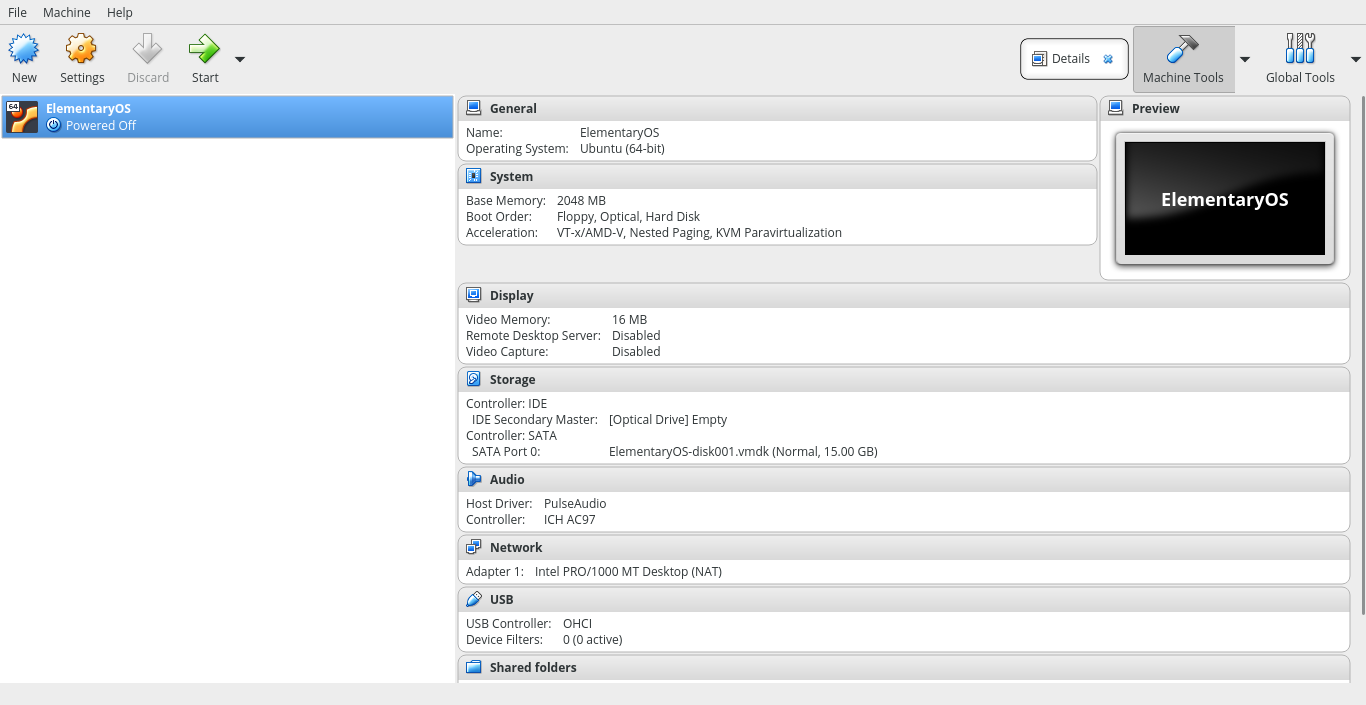
\includegraphics[scale=0.2]{figures/vbox.png}}
\end{center}
\end{frame}

\section{ElementaryOS}
\begin{frame}[fragile]
\pause\transdissolve

Click ``Start'' to start the machine

\pause\transdissolve\bigskip

Login as Uber Student (username \lstinline{student}) with password \lstinline{enigma}

\pause\transdissolve\bigskip

\begin{center}
\visible<4->{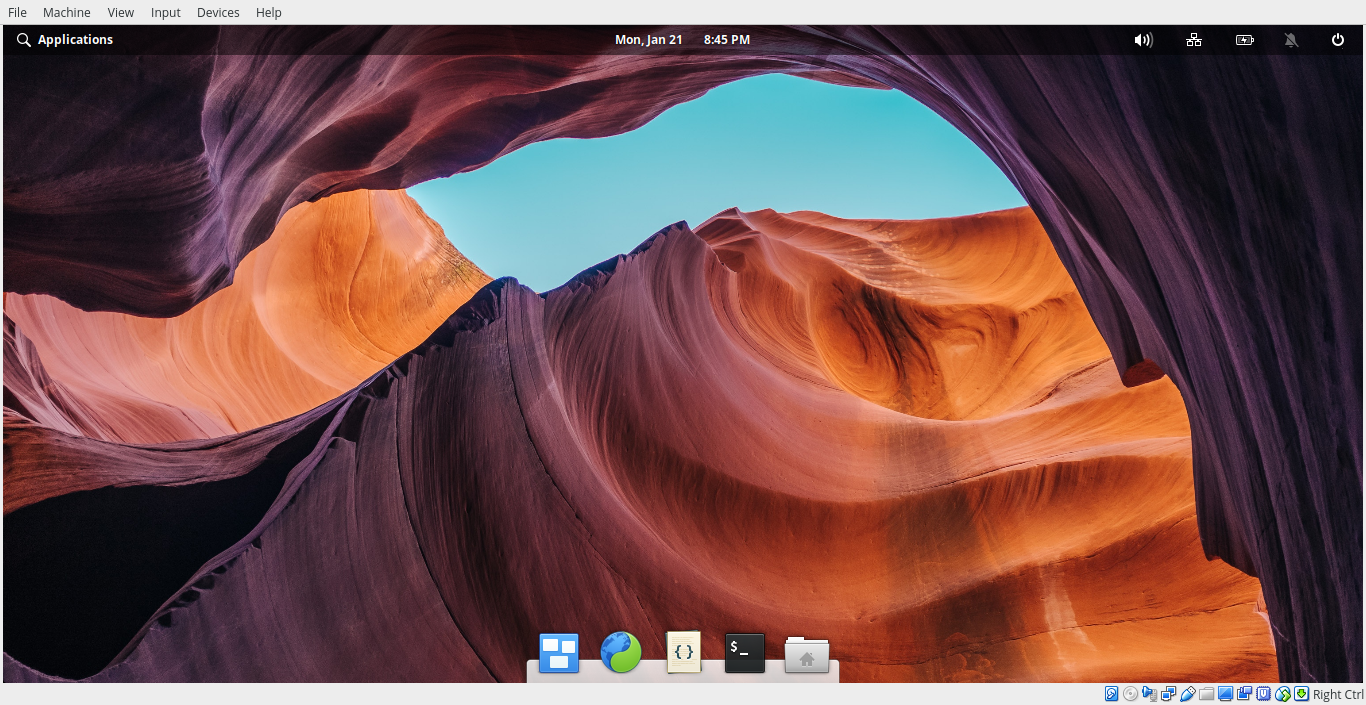
\includegraphics[scale=0.2]{figures/elementaryos.png}}
\end{center}

\pause\transdissolve\bigskip

To stop the machine, click \visible<5->{
\includegraphics[height=\myMheight]{figures/shutdown.pdf}} and select ``Shut Down...''
\end{frame}

\section{Tools}
\begin{frame}[fragile]
\pause\transdissolve

Web browser \visible<2->{
\includegraphics[height=\myMheight]{figures/web_browser.pdf}}

\pause\transdissolve\bigskip

Editor \visible<3->{
\includegraphics[height=\myMheight]{figures/editor.pdf}}

\pause\transdissolve\bigskip

Terminal \visible<4->{
\includegraphics[height=\myMheight]{figures/terminal.pdf}}

\pause\transdissolve\bigskip

File manager \visible<5->{
\includegraphics[height=\myMheight]{figures/file_manager.pdf}}
\end{frame}

\section{Editing Files}
\begin{frame}[fragile]
\pause\transdissolve

Use editor \visible<2->{
\includegraphics[height=\myMheight]{figures/editor.pdf}}

\smallskip

\begin{center}
\visible<2->{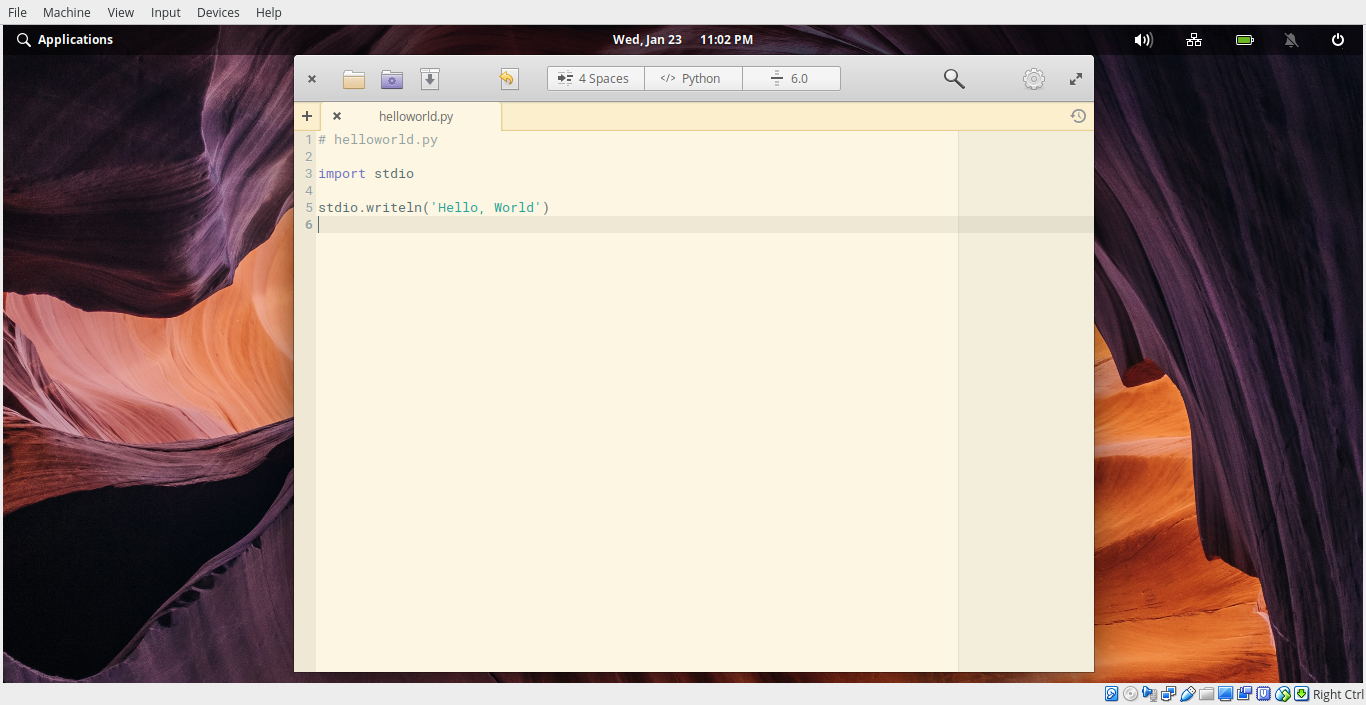
\includegraphics[scale=0.2]{figures/editing.png}}
\end{center}
\end{frame}

\section{Navigating the File System}
\begin{frame}[fragile]
\pause\transdissolve

Use file manager \visible<2->{
\includegraphics[height=\myMheight]{figures/file_manager.pdf}} and terminal \visible<2->{
\includegraphics[height=\myMheight]{figures/terminal.pdf}}

\smallskip

\begin{center}
\visible<2->{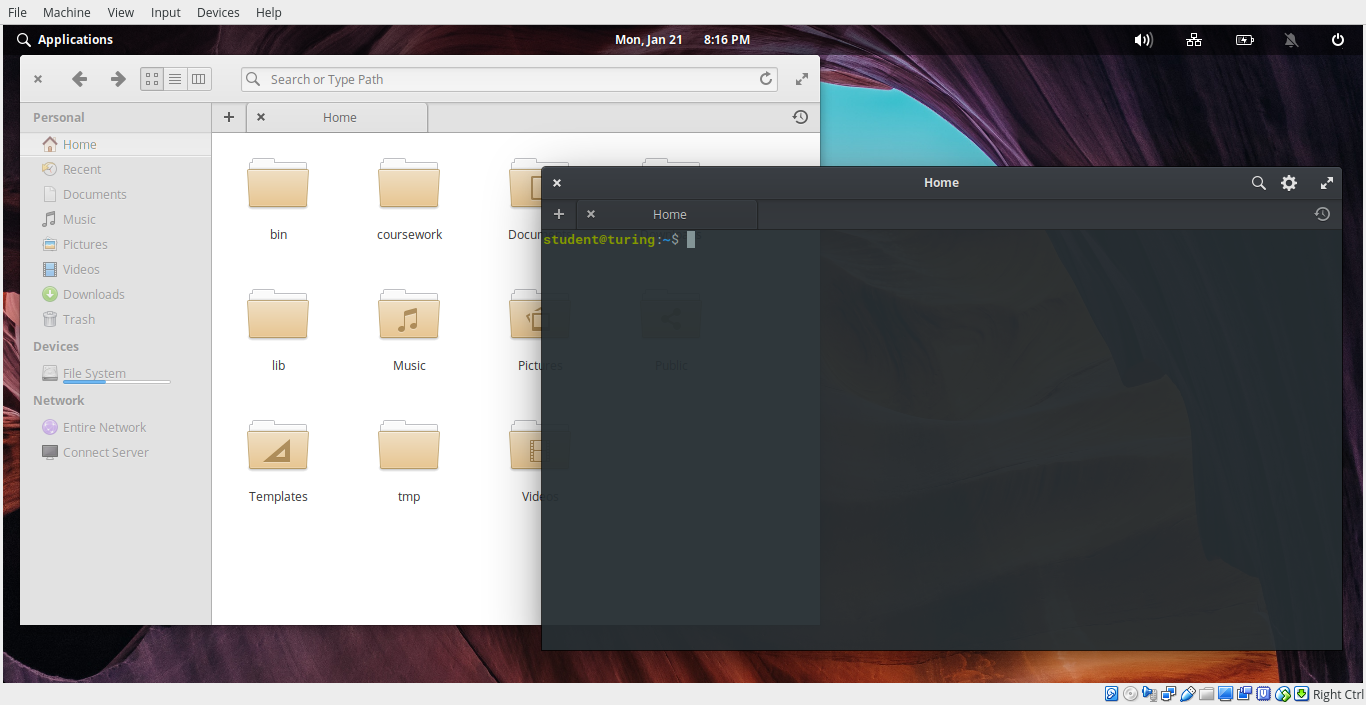
\includegraphics[scale=0.2]{figures/filesystem.png}}
\end{center}
\end{frame}

\section{Obtaining a Project}
\begin{frame}[fragile]
\pause\transdissolve

Launch terminal (opens in \lstinline{/home/student} by default)

\pause\transdissolve\bigskip

Change directory to \lstinline{coursework}

\begin{tcolorbox}[enhanced,drop shadow southwest,sharp corners,size=fbox,colback=black]
\begin{lstlisting}[style=terminal]
$ cd coursework
\end{lstlisting}
\end{tcolorbox}

\pause\transdissolve\bigskip

Download the project (eg, Project 1)

\begin{tcolorbox}[enhanced,drop shadow southwest,sharp corners,size=fbox,colback=black]
\begin{lstlisting}[style=terminal]
$ wget https://swamiiyer.net/cs110/project1.zip
\end{lstlisting}
\end{tcolorbox}

\pause\transdissolve\bigskip

Extract the downloaded zip file

\begin{tcolorbox}[enhanced,drop shadow southwest,sharp corners,size=fbox,colback=black]
\begin{lstlisting}[style=terminal]
$ unzip project1.zip
\end{lstlisting}
\end{tcolorbox}

\pause\transdissolve\bigskip

Remove the zip file

\begin{tcolorbox}[enhanced,drop shadow southwest,sharp corners,size=fbox,colback=black]
\begin{lstlisting}[style=terminal]
$ rm project1.zip
\end{lstlisting}
\end{tcolorbox}
\end{frame}

\section{Working on the Project}
\begin{frame}[fragile]
\pause\transdissolve

Change to the project directory (eg, \lstinline{project1})

\begin{tcolorbox}[enhanced,drop shadow southwest,sharp corners,size=fbox,colback=black]
\begin{lstlisting}[style=terminal]
$ cd project1
\end{lstlisting}
\end{tcolorbox}

\pause\transdissolve\bigskip

We are now under \lstinline{/home/student/coursework/project1}

\pause\transdissolve\bigskip

Run a program (eg, \lstinline{great_circle.py})

\begin{tcolorbox}[enhanced,drop shadow southwest,sharp corners,size=fbox,colback=black]
\begin{lstlisting}[style=terminal]
$ python3 great_circle.py 48.87 -2.33 37.8 -122.4
\end{lstlisting}
\end{tcolorbox}

\pause\transdissolve\bigskip

Check a program (eg, \lstinline{great_circle.py}) for coding style

\begin{tcolorbox}[enhanced,drop shadow southwest,sharp corners,size=fbox,colback=black]
\begin{lstlisting}[style=terminal]
$ pycodestyle great_circle.py
\end{lstlisting}
\end{tcolorbox}
\end{frame}

\begin{frame}[fragile]
\pause\transdissolve

Test your solutions for particular exercises/problems (eg, Exercise 1 and Problem 2)

\begin{tcolorbox}[enhanced,drop shadow southwest,sharp corners,size=fbox,colback=black]
\begin{lstlisting}[style=terminal]
$ python3 run_tests.py -v Exercise1 Problem2
\end{lstlisting}
\end{tcolorbox}

\pause\transdissolve\bigskip

Test your solutions for all exercises/problems

\begin{tcolorbox}[enhanced,drop shadow southwest,sharp corners,size=fbox,colback=black]
\begin{lstlisting}[style=terminal]
$ python3 run_tests.py -v
\end{lstlisting}
\end{tcolorbox}

\pause\transdissolve\bigskip

Use web browser \visible<4->{
\includegraphics[height=\myMheight]{figures/web_browser.pdf}} to sign on to Gradescope and upload your project files
\end{frame}
\end{document}
